\documentclass[10pt]{article}
\usepackage[letterpaper,margin=0.725in]{geometry}

\usepackage{fancyhdr}
\usepackage{amsmath}
\usepackage{mathtools}
\usepackage{hyperref}
\usepackage[english]{babel}
\usepackage{graphicx}
\usepackage{float}
\usepackage{caption}
\usepackage{amssymb}
\usepackage{amstext} % for \text macro
\usepackage{array}   % for \newcolumntype macro
\allowdisplaybreaks

\usepackage[T1]{fontenc}
\usepackage[numbered,framed]{matlab-prettifier}

\hypersetup{ colorlinks=true, linkcolor=blue}

\DeclareMathOperator{\atantwo}{atan2}
\newcolumntype{C}{>{$}c<{$}} % math-mode version of "l" column type

\pagestyle{fancy}
\lhead{RBE 500 - PA \#1 \newline Team 2: Peter Campellone, Aislin Hanscom, Christopher Poole}
\rhead{Due: 6/29/2021}

\begin{document}

\setlength{\abovedisplayskip}{6pt}
\setlength{\belowdisplayskip}{3pt}
\setlength{\abovedisplayshortskip}{4pt}
\setlength{\belowdisplayshortskip}{4pt}

\begin{enumerate}
	\item \textbf{Create the robot:}
	
	\begin{itemize}
		\item Spawn the robot to the ROS-Gazebo environment. Include and image of the robot.
		
		\item Include the robot definition file.
		\\
	\end{itemize}

	Include \href{http://wiki.ros.org/joint_state_publisher}{\texttt{joint\_state\_publisher}}
	
	Reference this \href{https://answers.ros.org/question/348008/connecting-gazebo-and-rviz/}{connecting-gazebo-and-rviz}
	\\
	
	To begin the simulation:
	\begin{itemize}
		\item \texttt{roslaunch rrbot\_gazebo rrbot\_world.launch}
	\end{itemize}	
	
	\item \textbf{Forward Kinematics:}
	Implement a FK node that
	
	\begin{itemize}	
		\item Subscribes to the joint values topic and reads them from the Gazebo simulator.
		\item Calculates the pose of the end-effector.
		\item Publishes the pose as a ROS topic (inside the callback function that reads the joint values).
	\end{itemize}
	Print the resulting pose to the terminal using the \texttt{rostopic echo} command and include a screenshot of the results.
	\\
	
	We begin by assigning coordinate frames to the manipulator:
	
	\begin{figure}[h]
		\centering
		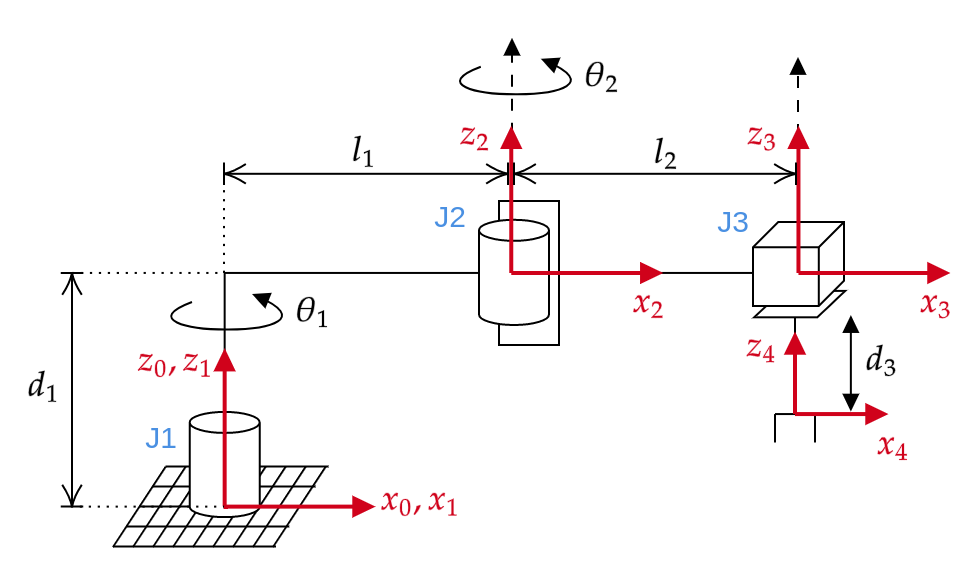
\includegraphics[width=0.6\textwidth]{figures/rrp_manipulator_reference_frames.png}
	\end{figure}
	
	We can then formulate the DH parameters coordinating to the links:
	
	\begin{center}
	\begin{tabular}{ c | C | C | C | C }
		Link & \theta_i & d_i & a_i & \alpha_i \\
		\hline 
		1 & \theta_1^* & d_1 & l_1 & 0 \\
		2 & \theta_2^* & 0 & l_2 & 0 \\
		3 & 0 & -d_3^* & 0 & 0 \\
	\end{tabular}
	\end{center}
	
	Next, we can calculate the transformations for each frame:
	
	\begin{align*}
		T_{i+1}^i &= \text{Rot}_z(\theta_i) \text{Trans}_z(d_i) \text{Trans}_x(a_i) \text{Rot}_x(\alpha_i) = \begin{bmatrix}
		\cos\theta_i & -\sin\theta_i \cos\alpha_i &\sin\theta_i \sin\alpha_i & a_i \cos\theta_i \\
		\sin\theta_i & \cos\theta_i \cos\alpha_i & -\cos\theta_i \sin\alpha_i & a_i \sin\theta_i \\
		0 & \sin\alpha_i & \cos\alpha_i & d_i \\
		0 & 0 & 0 & 1
		\end{bmatrix}
		\\
		T_{2}^1 &= \begin{bmatrix}
		1 & 0 & 0 & 0 \\
		0 & 1 & 0 & 0 \\
		0 & 0 & 1 & 0 \\
		0 & 0 & 0 & 1
		\end{bmatrix}
		\\
		T_{2}^1 &= \begin{bmatrix}
		\cos\theta_1 & -\sin\theta_1 \cos 0 &\sin\theta_1 \sin 0 & l_1 \cos\theta_1 \\
		\sin\theta_1 & \cos\theta_1 \cos 0 & -\cos\theta_1 \sin 0 & l_1 \sin\theta_1 \\
		0 & \sin 0 & \cos 0 & d_1 \\
		0 & 0 & 0 & 1
		\end{bmatrix} = \begin{bmatrix}
		\cos\theta_1 & -\sin\theta_1 & 0 & l_1 \cos\theta_1 \\
		\sin\theta_1 & \cos\theta_1 & 0 & l_1 \sin\theta_1 \\
		0 & 0 & 1 & d_1 \\
		0 & 0 & 0 & 1
		\end{bmatrix}
		\\
		T_{3}^2 &= \begin{bmatrix}
		\cos\theta_2 & -\sin\theta_2 \cos 0 &\sin\theta_2 \sin 0 & l_2 \cos\theta_2 \\
		\sin\theta_2 & \cos\theta_2 \cos 0  & -\cos\theta_2 \sin 0 & l_2 \sin\theta_2 \\
		0 & \sin 0 & \cos 0 & 0 \\
		0 & 0 & 0 & 1
		\end{bmatrix} = \begin{bmatrix}
		\cos\theta_2 & -\sin\theta_2 & 0 & l_2 \cos\theta_2 \\
		\sin\theta_2 & \cos\theta_2 & 0 & l_2 \sin\theta_2 \\
		0 & 0 & 1 & 0 \\
		0 & 0 & 0 & 1
		\end{bmatrix}
		\\
		T_{4}^3 &= \begin{bmatrix}
		\cos 0 & -\sin 0 \cos 0 &\sin 0 \sin 0 & 0 \cos 0 \\
		\sin 0 & \cos 0 \cos 0 & -\cos 0 \sin 0 & 0 \sin 0 \\
		0 & \sin 0 & \cos 0 & -d_3 \\
		0 & 0 & 0 & 1
		\end{bmatrix} = \begin{bmatrix}
		1 & 0 & 0 & 0 \\
		0 & 1 & 0 & 0 \\
		0 & 0 & 1 & -d_3 \\
		0 & 0 & 0 & 1
		\end{bmatrix}
	\end{align*}
	
	The combined transformation of the end effector is:
	\begin{align*}
		T_4^0 = T_1^0 T_2^1 T_3^2 T_4^3
	\end{align*}
	
	This calculation is used in the forward kinematic function \texttt{calc\_homogeneous\_transform(q)}:
	
\begin{lstlisting}[style=Matlab-editor,basicstyle=\mlttfamily,escapechar=`]
def calc_homogeneous_transform(q): # calculate the homogeneous transform from the base frame to EE
	# q = [th1, th2, d3]
	th1 = q[0]
	th2 = q[1]
	d3 = q[2]
	
	T1_0 = np.matrix([[1,0,0,0],[0,1,0,0],[0,0,1,0],[0,0,0,1]]) # frame 1 w.r.t 0
	T2_1 = np.matrix([[math.cos(th1),-math.sin(th1),0,l1*math.cos(th1)],[math.sin(th1),math.cos(th1),0,l1*math.sin(th1)],[0,0,1,d1],[0,0,0,1]])	# frame 2 w.r.t 1 
	T3_2 = np.matrix([[math.cos(th2),-math.sin(th2),0,l2*math.cos(th2)],[math.sin(th2),math.cos(th2),0,l2*math.sin(th2)],[0,0,1,0],[0,0,0,1]])	# frame 3 w.r.t 2 
	T4_3 = np.matrix([[1,0,0,0],[0,1,0,0],[0,0,1,-d3],[0,0,0,1]]) # frame 4 w.r.t 3
	
	T_EE = T1_0.dot(T2_1).dot(T3_2).dot(T4_3)
	
	return T_EE
\end{lstlisting}
	

	To run and test the subscriber/publisher function:
	
	\begin{itemize}
		\item Run \texttt{roslaunch scara\_gazebo scara\_world.launch}
		\item In a new window \texttt{roslaunch gazebo\_publish gazebo\_publish.launch} which allows the joint states to be published.
		\item In a new window \texttt{rostopic list} should show /scara/joint\_states
		\item \texttt{rostopic echo /scara/joint\_states} should show the joint states printing
		\item \texttt{rosrun scara\_forward\_kinematics configuration\_to\_operational\_sub.py} will run the program that subscribes to the joint states, calculates the forward kinematics, and publishes the end-effector pose back to the \texttt{Pose} topic. The print out can be seen below:
		
		\begin{figure}[h]
			\centering
			%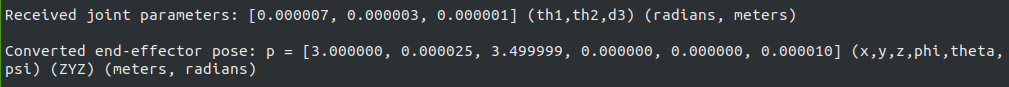
\includegraphics[width=0.6\textwidth]{figures/sub_pub_print_results.png}
		\end{figure}
	
		\item We can also see the \texttt{Pose} topic getting published by running \texttt{rostopic echo /scara\_robot/pose}
		
	\end{itemize}

	\item \textbf{Inverse Kinematics:}
	
	\begin{itemize}
		\item Implement an IK node (separate node) that has a service client that take a desired pose of the end effector and returns joint positions as a response.
	
		\item Test your node with \texttt{rosservice call}. Include a screenshot of the results.
	\end{itemize}

	The following definitions can be used to calculate the inverse kinematics:
	\begin{figure}[h]
		\centering
		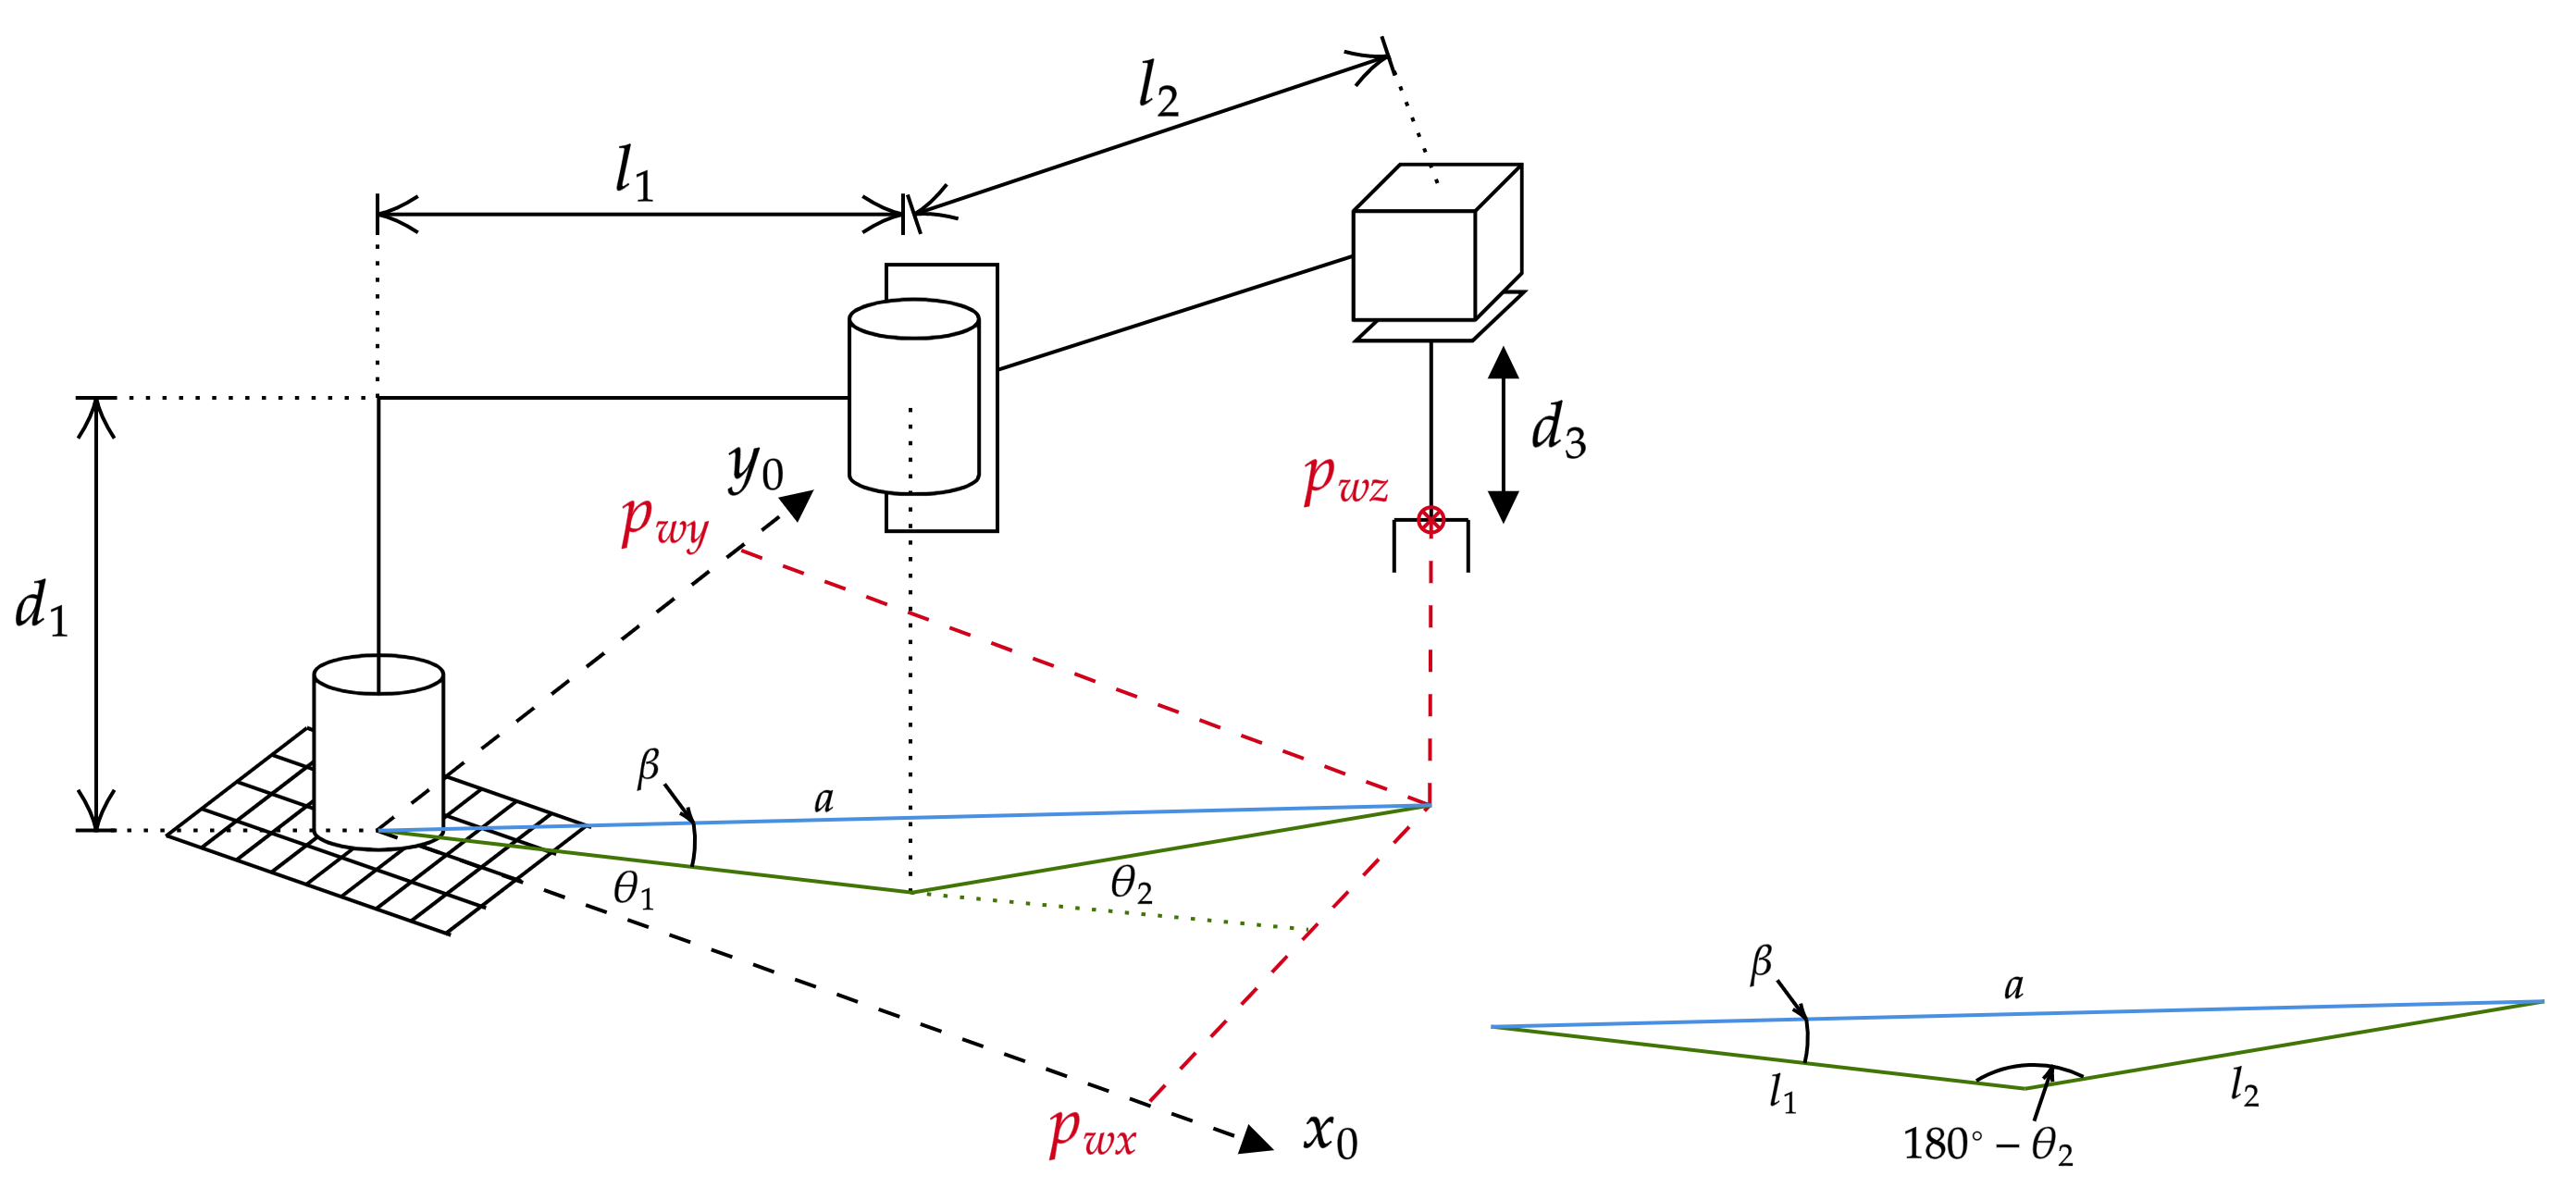
\includegraphics[width=0.8\textwidth]{figures/rrp_IK.png}
	\end{figure}
	\\
	The large right triangle can be used to calculate the following:
	\begin{align*}
		r &= \sqrt{p_x^2 + p_y^2} \\
		A &= \frac{p_x}{r} = \cos\alpha \Rightarrow
		\sin \alpha = \pm \sqrt{1 - A^2} \Rightarrow \alpha = \atantwo\left(\pm \sqrt{1-A}, A\right)
	\end{align*}
	\\
	The law of cosines can be used on the other triangle to calculate $\beta$ and $\theta_1$:
	\begin{align*}
		l_2^2 &= r^2 + l_1^2 - 2 r l_1 \cos\beta \\
		\cos\beta & = \frac{r^2 + l_1^2 - l_2^2}{2 r l_1} = C \Rightarrow \sin\beta = \pm\sqrt{1-C^2} \\
		\beta &= \atantwo\left(\pm\sqrt{1-C^2}, C\right) \\
		\theta_1 &= \alpha - \beta
	\end{align*}
	\\
	The law of cosines can be used again to calculate $\theta_1$:
	\begin{align*}
		r^2 &= l_1^2 + l_2^2 - 2 l_1 l_2 \cos(180-\theta_2) \\
		r^2 &= l_1^2 + l_2^2 + 2 l_1 l_2 \cos(\theta_2) \\
		\cos\theta_2 & = \frac{r^2 - l_1^2 - l_2^2}{2 l_1 l_2} = D \Rightarrow \sin\theta_2 = \pm\sqrt{1-D^2} \\
		\theta_2 &= \atantwo\left(\pm\sqrt{1-D^2}, D\right)
	\end{align*}
	\\
	Lastly, $d3$ is calculated simply as follows:
	\begin{align*}
		d_3 = d_1 - p_z
	\end{align*}
	\\
	The above equations are included in the server \texttt{inverse\_server.cpp}:
\begin{lstlisting}[style=Matlab-editor,basicstyle=\mlttfamily,escapechar=`]
double D = - (((l1*l1)+(l2*l2)-(x*x+y*y))/(2*l1*l2));
double C = (((l1*l1)+x*x+y*y-(l2*l2))/(2*l1*sqrt(x*x+y*y)));

double B = sqrt(1-D*D);
double E = sqrt(1-C*C);

double alpha = atan2(y, x);

res.theta1 = alpha-atan2(E, C);
res.theta2 = atan2(B, D);
res.d3 = d1 - z;
\end{lstlisting}
\end{enumerate}
\end{document}



